\vspace{-1mm}
\section{Conclusion and Future Avenues}
\vspace{-1mm}
%In this paper, we define different orientations and categories of hallucinations holistically. We introduce a large-scale hallucination benchmark corpus called 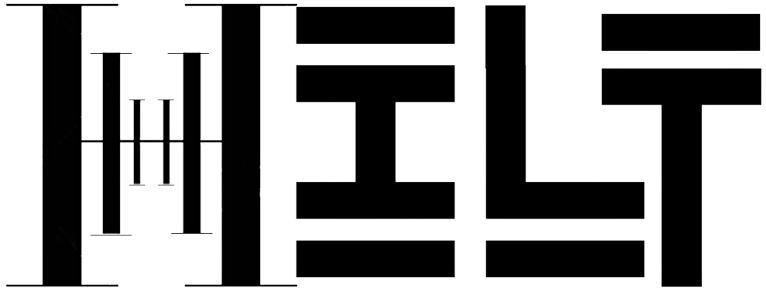
\includegraphics[height=0.3cm,width=1cm]{img/hilt.png}. We also propose a new evaluation metric called \textit{Hallucination Vulnerability Index (HVI)} to measure the extent of hallucinations in the text generated by LLMs. Lastly, we examine two families of mitigation techniques, namely ENTROPY\textsubscript{BB} and FACTUALITY\textsubscript{GB}, that aim to alleviate hallucination. These techniques can serve as baselines for future researchers interested in utilizing the 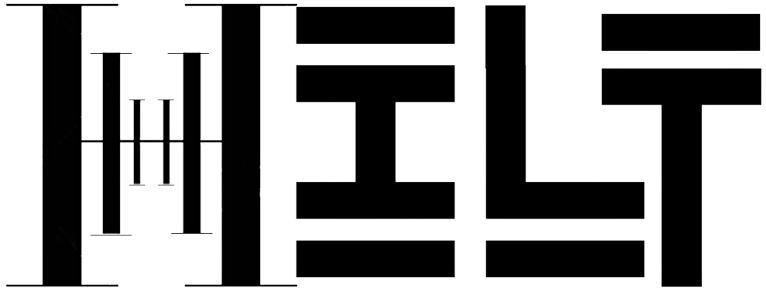
\includegraphics[height=0.3cm,width=1cm]{img/hilt.png} dataset to study hallucination.

The enthusiasm and achievements surrounding LLMs have led to their widespread adoption, and this trend is only expected to flourish. However, one of the most significant challenges faced by LLMs today is hallucination. In light of this, 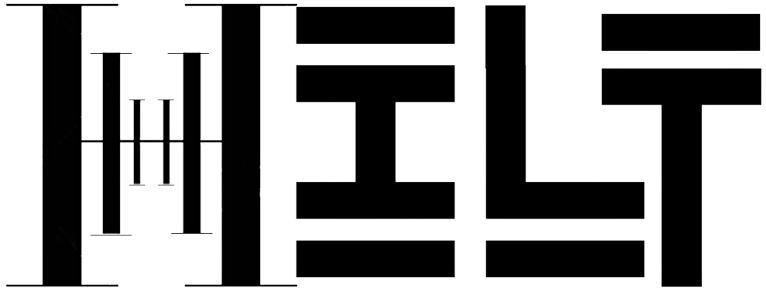
\includegraphics[height=0.3cm,width=1cm]{img/hilt.png} benchmark and \textit{\ul{Hallucination Vulnerability Index (HVI)}} will continue to serve the wider scientific community and aid policy-makers. 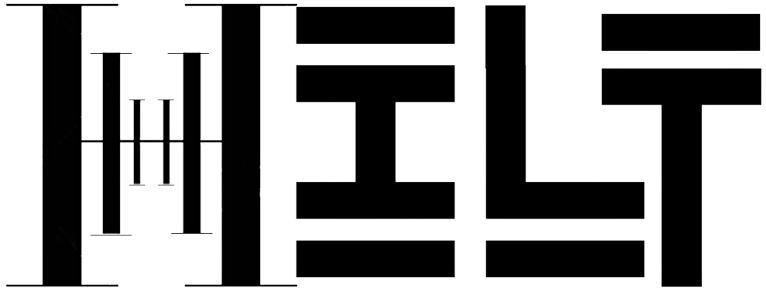
\includegraphics[height=0.3cm,width=1cm]{img/hilt.png} benchmark and \textit{HVI} will be publicly open for further collaborative updates. Two proposed mitigation techniques can serve as baselines.
%We introduce a first-of-its-kind large-scale hallucination benchmark corpus called 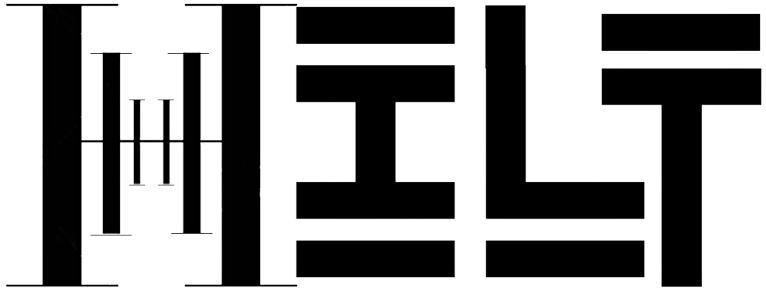
\includegraphics[height=0.3cm,width=1cm]{img/hilt.png}. 
%Two proposed mitigation techniques ENTROPY\textsubscript{BB} and FACTUALITY\textsubscript{GB}, can serve as baselines.
%for future researchers interested in utilizing the 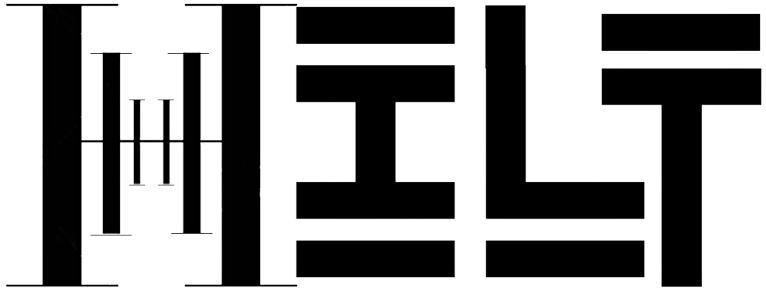
\includegraphics[height=0.3cm,width=1cm]{img/hilt.png} benchmark to study hallucination.
%In the future, we shall work on improving both hallucination detection and mitigation methods. One plausible line of direction would be injecting external knowledge to mitigate such hallucinations. 

